%%%%%%%%%%%%%%%%%%%%%%%%%%%%% PACKAGES %%%%%%%%%%%%%%%%%%%%%%%%%%%%%%%%%%
\documentclass[11pt, letterpaper]{article} % Customise character size
\usepackage{graphicx} % Required for inserting images
\usepackage{lineno} % line numbers
\usepackage{setspace} % set space width between columns
\usepackage[authoryear]{natbib} % Bibliography styles
    \bibliographystyle{agsm}
\usepackage[margin = 2cm]{geometry} % Custom margin
\usepackage[utf8]{inputenc} 
\usepackage{multirow} % Better tables - combine cols and rows
\usepackage{booktabs} % Better tables
  \setlength\heavyrulewidth{0.20ex}
  \setlength\cmidrulewidth{0.10ex}
  \setlength\lightrulewidth{0.10ex}
\usepackage[font=normalsize,labelfont={bf}]{caption} % make captions further from the table
  \captionsetup[table]{aboveskip=3pt}
\usepackage{siunitx} % mathematical operators

\usepackage{helvet} % Helvetica font
\renewcommand{\familydefault}{\sfdefault} % Set default as Helvetica


\begin{document}

% ---------------------------------------------------------------- %
%%%%%%%%%%%%%%%%%%%%%%%%%%%%% TITLE PAGE %%%%%%%%%%%%%%%%%%%%%%%%%%%
% ---------------------------------------------------------------- %

\begin{titlepage}
    
\includegraphics[width=4cm]{logo_new.png} % Imperial logo
    
    \centering
    
    % Title
    \vspace{3.5cm}
    \Huge
    \textbf{Comparing machine learning algorithms for automatic pigeon behaviour categorisation}
    
    % Author
    \vspace{2cm} % Adjust vertical space
    \huge % Change text size
    \textbf{Tianle Shao} \\

    \vspace{0.5cm}
    \Large
    August 2024

    % other information
    \vspace{6cm} % Adjust vertical space
    \normalsize
    Word Count: 5256 \\
    \vspace{1cm}
    A thesis submitted in partial fulfilment for the degree of \\
    Master of Science at Imperial College London \\

    \vspace{1cm}
    \textit{Submitted for MSc Computational Methods in Ecology and Evolution} \\

\end{titlepage}


% ---------------------------------------------------------------- %
%%%%%%%%%%%%%%%%%%%%%%%%% DECLARATION & ACKNOWLEDGEMENTS %%%%%%%%%%%
% ---------------------------------------------------------------- %

\doublespacing
\section*{Declaration}

I declare that I am the sole author of this thesis. The keypoint data used in this project originates from the 3D-POP dataset, and is freely available to download online in csv format. The corresponding behaviour ground truth data can be obtained using the methodology detailed in \citet{delacoux_fine-scale_2024}. The code used for normalisation of coordinates was adapted from code by Alex Chan. I was responsible for all other data manipulation, coding, model training and write-up for this thesis.

% ---------------------------------------------------------------- %
%%%%%%%%%%%%%%%%% ABSTRACT %%%%%%%%%%%%%%%%%%%%%%%%%%%%%%%%%%%%%%%%%
% ---------------------------------------------------------------- %

\newpage
%\linenumbers
    
\section{Abstract}

    Machine learning algorithms offer a quick and unbiased way of classifying behaviours from corresponding posture data of an animal, reducing the need for manual classification, and providing valuable information for fields from neuroscience to animal welfare. However, what remains unclear is the optimal type of posture features and the appropriate time frame to best capture and predict these behaviors.
    %
    In this study, I compare 2D keypoints, 3D keypoints, and 3D keypoint-derived angles as approximations of pigeon posture across 1-90 frames of time, to evaluate the predictive accuracy of different machine learning models.
    %
    I find that using 3D keypoint data over 30-60 time frames yielded the highest prediction accuracy. 
    %
    3D keypoints can capture depth information, full range of motion and are not vulnerable to occlusions. 30-60 frames correspond to 1-2 seconds, which gives insight on the optimal time frame to capture behavioural motions in pigeons. These findings highlight the potential of using 3D tracking with temporal components for more accurate animal behaviour classification. Despite this, overall accuracy was low across all models, potentially indicating problems with high dimensionality in the data samples, or that the algorithms are not suitable for time series classification.
    
    

% ---------------------------------------------------------------- %
%%%%%%%%%%%%%%%%% INTRO %%%%%%%%%%%%%%%%%%%%%%%%%%%%%%%%%%%%%%%%%
% ---------------------------------------------------------------- %
\section{Introduction}
    
    %---- Overview of animal behaviour - studies & importance ---------%
    Animals exhibit a diverse range of behaviours - from the walking or resting of an individual, to complex social/collective behaviours involving groups of animals \citep{collective_2005, hughey_challenges_2018}, and cryptic fine scaled behaviours that can be difficult to observe and recognise by eye (D.D. Brown et al., 2013). How an animal behaves can give insight on its neurobiology, physiology, health and social relations, which provides crucial information to fields such as neuroscience \citep{datta_computational_2019, mathis_deeplearning_2020}, conservation \citep{panda_2021}, agriculture \citep{locust_2024} and animal welfare \citep{animal_welfare_2016}. However, the study of animal behaviour has traditionally relied heavily on, and has been limited by the need for extensive manual observation and classification of data \citep{anderson_comp_ethology_2014}. Two of the main challenges of human labour are the difficulties of obtaining sufficient observational data by eye, and the subjective and unreliable nature of manual human classification of behaviours \citep{anderson_comp_ethology_2014, segalin_mouse_2021}. \\
    
    %---- Data collection for animal behaviour ----------------------------%
    \noindent The challenge of obtaining sufficient high-quality observational data has become less problematic in recent years. In many cases, it is no longer necessary for scientists to manually keep track of wild animals, as the process of data collection has been made more convenient by technological advancements, including in camera technology, remote sensing \citep{torney_caribou_remotesensing_2018} and bio-logging instruments such as mounted GPS \citep{kays_GPS_2015} and accelerometers (D.D. Brown et al., 2013). Similarly for more controlled and lab-based studies, technologies such as motion capture can not only automate data collection, but also capture data at increasingly fine scales \citep{nagy_smart-barn_2023}. 
    With these technologies at hand, researchers are able to track animals at high resolution over prolonged periods \citep{hughey_challenges_2018}, which provides extensive data, image and video footage. At the finest scale, the specific postures of individual animals can be captured, providing researchers with opportunities to analyse behaviour at a scale not previously possible. \\

    
    %---- Machine learning ------------------------------------------------%
    \noindent Despite the large amount of usable data on animal features such as posture, the process of classifying this raw data into behaviours has remained the greatest challenge \citep{hughey_challenges_2018}. For this, machine learning has emerged as the main approach in automatic behavioural classification -- the process of analysing raw data and classifying behaviours from it. Machine learning methods are hypothesis-free, and do not require biologically relevant data distributions to be fit to it, instead iterating to find a model that best fits the data \citep{ML_for_behaviour_2017}. This prioritisation of prediction over having a biologically meaningful underlying hypothesis means machine learning methods excel at predicting complex datasets, but often at the expense of interpretability of the constructed models \citep{ML_for_behaviour_2017}. Numerous different algorithms with a range of methodologies have become available to automatically classify animal behaviours, from classic support vector machines and decision trees \citep{bergen_review_2023} to complex unsupervised clustering \citep{hsu_b-soid_2021} and computer vision algorithms \citep{bohnslav_deepethogram_2021}. \\
    %
    % Popular algorithms for behavioural prediction include supervised methods such as support vector machines, decision trees and neural networks, which are provided pre-classified data to predict \citep{wittek_supervised_2023}. Unsupervised methods such as clustering and dimensionality reduction are not given classified data, and instead generate classifications based on observed trends or clustering in data \citep{hsu_b-soid_2021}. A combination of supervised and unsupervised methods have also been used recently \citep{tillmann_A-soid_2024}. \\

    
    %-------------------------------------------------------------------------%
    \noindent Images and videos can capture a large range of animal posture and movement features, however there is no consensus on what features to use, and how these features should be extracted to maximise the accuracy when predicting behaviours using machine learning algorithms \citep{behav_across_scales_2018}. This is particularly true for posture tracking of individual animals, as keypoints that estimate posture vary widely in form, and it remains unclear whether they should be represented in 2D, 3D or a different format entirely \citep{pereira_quantifying_2020, mathis_deeplearning_2020}.
    %
    Many studies have made use of 2D keypoints, as they are relatively easy to mark manually, needing only images or videos of animals. They have also become easier to predict due to increasingly mature and powerful tools such as DeepLabCut \citep{mathis_deeplabcut_2018} and LEAP \citep{LEAP_2019}, which are capable of automatically extracting keypoint information from images and videos of multiple animals, using only a small manually labelled dataset to train. In contrast, 3D keypoints are more difficult to obtain, as they often require prior setup of multiple camera views or motion capture systems to calculate accurate 3D coordinates \citep{joska_acinoset_2021, waldmann_3d-muppet_2023}. However, since they make use of a greater range of viewpoints, 3D keypoints are less vulnerable to occlusions, can better capture the postures of flexible animals such as mice \citep{pereira_quantifying_2020}, and can define the fine scale movement of limbs and appendages \citep{3D_macaque_2020, 3D_monkey_2023}. Keypoints can also be further modified in an attempt to not only simplify the data, but also extract key features that give more information on posture. As keypoints often represent specific body locations like joints, the angles of those joints can be calculated to approximate animal posture \citep{raspa_studying_2021, ferres_predicting_2022}, offering an alternative to keypoints. While each data type has its advantages and disadvantages, few studies have directly compared 2D, 3D, and angle data for behavioral prediction. It therefore remains unclear whether traditional 2D keypoints are sufficient for prediction, if the extra effort required in obtaining 3D keypoints produces more accurate results, or if modification from keypoint to angle data would produce the best outcomes. \\
    
    \noindent Additionally, many behaviours are not stationary, consisting of temporal components which may not be accurately predictable using stationary images \citep{datta_computational_2019}. These temporal components include repetitive/cyclic movements over time, such as head bobbing of pigeons when walking \citep{head-bobbing_1988} or the wave-like crawling motion of the roundworm C. elegans (A.E.X. Brown et al., 2013). Repetitive movements can contain many fine scaled micro-movements, or motifs, the duration of which can vary widely depending on their complexity. This brings into question the optimal duration of time a recording should be to capture these movements, and whether this time is better allocated for full behaviours as classified by human eye, or optimised for detecting shorter motifs that make up full behaviours. Studies on humans have found that time frames of 2 seconds or less give the best trade-off between accuracy and prediction speed for behaviours \citep{banos_window_2014}. Although some equivalent research has been done for animals, the behaviours of different species vary greatly, and it remains unclear if optimal time scales found for one species can be generalised across species. \\

    
    
    %-------------------------------------------------------------------------%
    \noindent In this project, I attempt to fill these gaps in knowledge by comparing how differing posture estimation data types and sample time scales can affect the classification accuracy of machine learning algorithms. 
    %
    To test this, I made use of the 3D-POP dataset, a large dataset with posture data of freely-moving pigeons recorded at 30 frames per second \citep{naik_3d-pop_2023}. This dataset is unique in that posture is provided in the form of both 2D and 3D keypoints, with the corresponding behavioural annotations of all individual pigeons at any given time frame. I tested and compared the effectiveness of 2D keypoints, 3D keypoints and angles derived from 3D keypoints for behavioural prediction, to determine which data type grants a higher prediction accuracy.
    %
    Additionally, I tested how the length of time captured for each behaviour sample affected prediction accuracy. This was done by varying the number of subsequent time frames each sample covers, from a single frame, representing 1/30 of a second, to 90 consecutive frames, representing 3 seconds.
    %
    Finally, I tested if reducing complexity and dimensionality of my data affected prediction accuracy, as more complex data is more difficult for machine learning algorithms to predict. This modification was done to each sample by conserving the overall time frame of a sample, but removing frames at set intervals so that only 15, 10 or 5 frames remain. 
    %
    Two powerful machine learning algorithms were used to fit all data, namely the random forest \citep{breiman_randomforest_2001} and the Extreme Gradient Boosting (XGBoost) \citep{chen_xgboost_2016} algorithms.
    
    
    

% ---------------------------------------------------------------- %
%%%%%%%%%%%%%%%%% METHODS %%%%%%%%%%%%%%%%%%%%%%%%%%%%%%%%%%%%%%%%%
% ---------------------------------------------------------------- %
\section{Methods}

    \begin{figure}
        \centering
        \includegraphics[width=1\linewidth]{angle_location_figure.pdf}
        \caption{\textbf{a.} Position of the 9 keypoints on the body of pigeons, and the 2 rigid bodies that are formed by them \textbf{b.} Position of 3D angles on the body of pigeons, and the points and vectors they were calculated from.}
        \label{fig:pigeon_kp}
    \end{figure}

    
    \subsection{Experimental Dataset}

    For this study, I used the 3D-POP dataset \citep{naik_3d-pop_2023}, which contains 6 hours of video footage of freely moving pigeons tracked by a motion capture system at 30 frames per second. The footage is split into 59 trials - independent recordings of pigeon flocks, with either 1, 2, 5 or 10 individuals. The motion capture system provides the basis for keypoint prediction, which estimates the posture of individual pigeons in the form of 2D and 3D keypoints.
    %
    Each pigeon is defined by 2 rigid bodies - the head and the body. 9 keypoints are predicted overall, with 4 keypoints on the head - beak, nose, left eye and right eye, and 5 keypoints on the body - top keel, bottom keel, left shoulder, right shoulder and tail (figure \ref{fig:pigeon_kp}a). keypoints on these rigid bodies are assumed to be fixed in relation to each other, but keypoints on different rigid bodies can move in relation to each other. \\
    
    \noindent The corresponding ground truth for pigeon behaviours was defined by \citet{delacoux_fine-scale_2024}, where the behavioural classifications were obtained using a combination of manual human annotation, and by using simple thresholds to classify keypoints. Behavioural ground truth is available for all frames of footage for all individuals, with each frame of each individual bird corresponding to one or more of 11 total types of behaviour.
    %
    The behaviours were classified as either behaviours instances (head down, vigilance status, pecking, grooming, walking, flying, bowing), which could occur without dependency on other behaviours, 
    or behavioural states (courting status, courted status, bowing status, feeding), which could only occur depending on the occurrence of other behaviours. For instance, the occurrence of `feeding' would be dependent on the occurrence of two or more `pecking' instances within 6 seconds.


    \begin{figure}
        \centering
        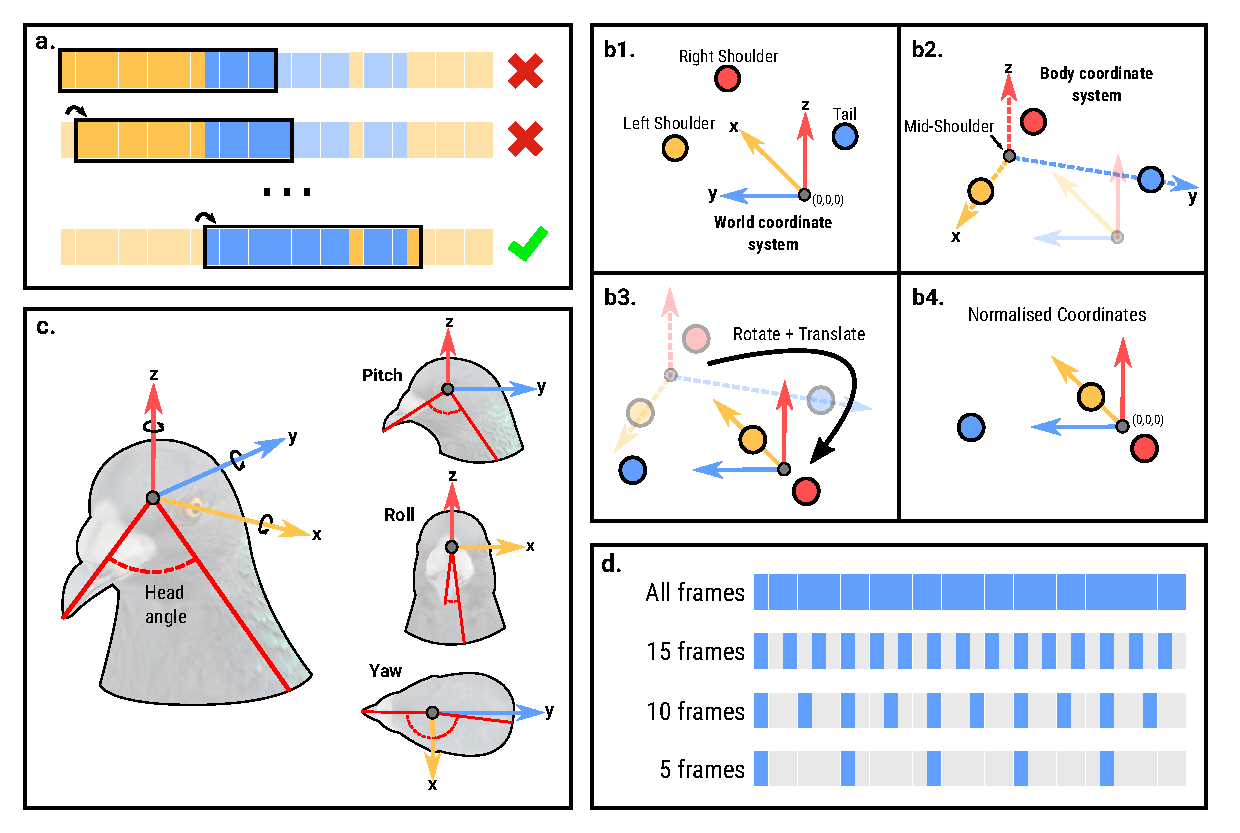
\includegraphics[width=1\linewidth]{methods_diagram.pdf}
        \caption{Overview of data pre-processing steps. \textbf{a.} The sliding window approach to detect continuous frames of behaviour, where blue are frames of a desired behaviour. \textbf{b.} Normalisation of 3D keypoint coordinates. \textbf{1.} Normalisation acts on the left/right shoulders and tail keypoints of each pigeon. \textbf{2.} The body coordinate system is created by centering the x, y and z axes at the mid-shoulder point, with the z-axis as the vector normal of the plane created by the shoulders and tail keypoints, the y-axis going through the tail point, and the x-axis perpendicular to both the x and y axes. \textbf{3.} The rotation and translation needed to align the body and world coordinate systems is calculated and applied to all keypoints, including those not depicted. \textbf{4.} The body and world coordinate systems are fully aligned. \textbf{c.} The head angle in 3D, broken down into its pitch, roll and yaw components. The same is done to the neck angle. \textbf{d.} Process of subsetting a set of continuous frames, in this case 30 frames, into subsets of 15, 10 and 5 non-continuous frames (blue frames).}
        \label{fig:methods_overview}
    \end{figure}


    \subsection{Data pre-processing}

    All data pre-processing was carried out using Python version 3.10.12. The following data pre-processing steps were done for both the training and testing datasets, which have been pre-defined by the 3D-POP dataset. The training dataset was used to train the machine learning algorithms, whereas the testing dataset was used to test the accuracy of algorithms after they have been fully trained.

        \subsubsection{Sampling data for continuous behaviour}
        Data trials with only 1 pigeon were not used, as pigeons in these trials tended to exhibit less varied behaviour than trials with more pigeons, contributing to behaviours such as `vigilance status' that were already abundant in other trials. This could be due to larger groups offering greater predator detection, and therefore allowing individuals to exhibit behaviours other than vigilance \citep{beauchamp_what_2008}.
        For data trials with flocks of 2, 5 and 10 pigeons, the behaviour and keypoint information of individual pigeons were extracted and analysed separately. Each row of keypoint and behaviour were assigned unique IDs.
        %
        I found chunks of behaviour that were continuous for 90 frames (3 seconds) by using a sliding window approach, an extensively used approach for characterising behaviours \citep{banos_window_2014,fly_timeseries_2019}, to examine each individual bird of each trial separately (figure \ref{fig:methods_overview}a). Continuous behaviour was defined as having over 70\% of all behaviours within a given sliding window to be the same as the first behaviour in the window, and fewer than 1/3 of all behaviours corresponding to `N/A' keypoint data. This was necessary due to inaccuracies resulting from the motion capture system. The remaining missing values for each sample were interpolated using a linear function. \\
        
        \noindent 7 behaviour classes were selected to be used - grooming, courting status, bowing status, head down, feeding, walking and vigilance status. The `courted status' behaviour was not used as interactions between individuals were not considered in this study, and the behaviour otherwise appears the same as walking. The remaining behaviours were not used as they were rarely continuous for 90 frames, and offered too few samples.
        %
        To ensure the sample size of each behaviour class was balanced, the behaviour with the smallest available sample size was identified, and the sample sizes of all other behaviours were reduced to match the smallest sample size, resulting in fully balanced classes.

        \subsubsection{Normalisation of coordinates}
        Coordinates were normalised to provide consistency of scale, position and orientation between different samples. This was done by creating a separate coordinate system centered on the pigeon's body, alongside the existing world coordinate system centered on the (0, 0, 0) or (0, 0) point. For the body coordinate system, the x, y and z-axes were centered at the midpoint between the left and right shoulder (mid-shoulder) keypoints. The z-axis was the vector normal to the plane formed by the left/right shoulder and tail keypoints. The y-axis was parallel to the plane, and passes through the tail keypoint. The x-axis points in the direction of the left shoulder keypoint, and is perpendicular to both the z and y-axes. The rotation and translation needed for the body coordinate system to become overlaid with the world coordinate system was calculated, and all keypoints were moved accordingly. This centers the mid-shoulder at world coordinate position (0, 0, 0) for 3D keypoints (figure \ref{fig:methods_overview}b). For 2D keypoints, the 3D y and z-axes in the body coordinate system are replaced by the x and y-axis, whereas the 3D x axis does not exist. The mid shoulder keypoint is centered at world coordinate position (0, 0). 
        %
        This process however would have eliminated any indication of movement between frames, giving the need to calculate the speed of movement between frames for individual pigeons. This was done by calculating the Euclidean distance between the bottom keel points of subsequent frames before normalisation was carried out.

        \subsubsection{Creating the angle dataset}
        Given that the body was aligned in all pigeons through normalisation of coordinates, a pigeon's further movement is limited to the rotation of the head and neck. Two 3D angles were calculated from the 3D keypoint dataset to represent the rotation of the head and neck. These angles were derived from 4 specific keypoints: the beak, the tail, the midpoint between the left and right eyes (mid-eye), and the midpoint between the left and right shoulders (mid-shoulder). The vertex of the head angle was the mid-eye point, with the sides extending to the beak and mid-shoulder points. The vertex of the neck angle was the mid-shoulder point, with the sides extending to the mid-eye and tail points (figure \ref{fig:pigeon_kp}b).
        % -------------------------------------------------------------------- %
        However, angles themselves are relative and do not give any absolute directional indication. For instance, the head pointing forwards and backwards could have the same angle. To address this, both the head and neck angles were broken down into their pitch, roll and yaw components to capture movement in the x, y and z planes separately. Pitch, roll and yaw angles in degrees were calculated by removing x, y and z coordinates respectively, and calculating the angles on the resulting 2D planes (figure \ref{fig:methods_overview}c).

        \subsubsection{Data subsets}
        
        The 90 frame samples were truncated to 60, 30, 15 and 1 frame, to compare how the length of time each sample corresponds to changes prediction accuracy.
        Due to the 30 fps framerate, each second of data contains many frames. However, individual postures in consecutive frames are unlikely to vary greatly, resulting in model inputs containing many features. To reduce data redundancy whilst also capturing larger changes in posture and movement, The 90, 60 and 30 frame samples were subsetted by extracting frames at set intervals so that only 15, 10 or 5 frames remain (figure \ref{fig:methods_overview}d). The 15 frame samples were subsetted so that 5 frames remain.
        %
        Datasets were flattened into a vector to be inputted into the models. Additionally, the movement speed data calculated beforehand was added to this data vector.


    \subsection{Automatic behaviour classification}

        \subsubsection{Machine learning algorithms}
        To test how the different data affected performance of machine learning algorithms, I fitted random forest \citep{breiman_randomforest_2001}, an ensemble classification tree algorithm, and Extreme Gradient Boosting (XGBoost) \citep{chen_xgboost_2016}, a boosted classification tree algorithm algorithms to the dataset. Both of these algorithms are built to be robust to overfitting, and have proven to be not only powerful but also efficient in animal behaviour prediction \citep{rf_vs_xg_2019}. 
        All algorithms were fit in Python version 3.10.12. I used the ``scikit-learn" package \citep{scikit-learn} to fit the random forest algorithm, and the ``XGBoost" package to fit the XGBoost algorithm. All models were fit with default parameters, and the random seed was set to 69 for all models to ensure repeatability. The model that achieved the highest predictive accuracy was fine tuned  with a hyperparameter tuning grid search, and 5-fold cross validation to maximise performance. To test if sample size had an impact on the prediction accuracy, I trained the best performing model using a range of different sample sizes and used it to predict the same test set. To test the relationship between sample size and prediction accuracy, an asymptotic regression model was fitted to the data using non-linear least squares. (Figure \ref{fig:model_performance}).

        \subsubsection{Statistical testing}
        All statistical analysis was carried out using R version 4.1.2.
        To explore the effect of model, keypoint data type, total time frame and subsetted time frame on prediction accuracy, a multi-way analysis of of variance (ANOVA) was performed. Prediction accuracy was the response variable, with model, keypoint data type, total time frame and subsetted time frame as the categorical explanatory variables, with 2, 3, 5 and 4 levels respectively. All assumptions of the model were examined through diagnostic plots, and found to be satisfied. A post-hoc Tukey test was used to detect pairwise differences between different levels of each categorical explanatory variable. 



% ---------------------------------------------------------------- %
%%%%%%%%%%%%%%%%% RESULTS %%%%%%%%%%%%%%%%%%%%%%%%%%%%%%%%%%%%%%%%%
% ---------------------------------------------------------------- %
\section{Results}


\begin{table}[htbp]
    \centering
    \caption{Accuracy scores of all models with each combination of model, data type, total frame length, and frame length after subsetting. The highest score for each model and datatype combination is highlighted in bold.}
    \begin{tabular}{cccccccccccc}

    \toprule
    \multicolumn{3}{c}{} & \multicolumn{4}{c}{\textbf{Random forest}} & \multicolumn{1}{c}{} & \multicolumn{4}{c}{\textbf{XGBoost}}\\ 
    \multicolumn{3}{c}{} & \multicolumn{4}{c}{Frames after subset} & \multicolumn{1}{c}{} & \multicolumn{4}{c}{Frames after subset}\\ 
    \cmidrule(rl){4-7} \cmidrule(rl){9-12}
    &Total frames && All     & 15     & 10     & 5     & & All     & 15     & 10     & 5 \\ 
    \cmidrule(rl){2-2} \cmidrule(){4-7} \cmidrule(){9-12}
    \multirow{5}{*}{\textbf{2D KP}} &90 &&0.220 &0.216 &0.233 &0.196 &&0.184 &0.216 &0.192 &0.192 \\
&60 &&0.216 &0.212 &0.229 &0.233 &&\textbf{0.257} &0.216 &0.176 &0.167 \\
&30 &&\textbf{0.249} &0.200 &0.229 &0.171 &&0.196 &0.196 &0.188 &0.192 \\
&15 &&0.208 &--- &--- &0.220 &&0.151 &--- &--- &0.151 \\
&1 &&0.237 &--- &--- &--- &&0.204 &--- &--- &--- \\
    \cmidrule(rl){2-2} \cmidrule(){4-7} \cmidrule(){9-12}
    \multirow{5}{*}{\textbf{3D KP}} &90 &&0.327 &0.306 &0.310 &0.286 &&0.290 &0.249 &0.265 &0.257 \\
&60 &&0.253 &0.269 &0.290 &0.273 &&0.302 &0.302 &0.298 &0.286 \\
&30 &&\textbf{0.355} &0.327 &0.318 &0.335 &&0.282 &\textbf{0.335} &0.310 &0.302 \\
&15 &&0.294 &--- &--- &0.286 &&0.265 &--- &--- &0.282 \\
&1 &&0.261 &--- &--- &--- &&0.310 &--- &--- &--- \\
    \cmidrule(rl){2-2} \cmidrule(){4-7} \cmidrule(){9-12}
    \multirow{5}{*}{\textbf{Angles}} &90 &&0.233 &0.208 &0.204 &0.208 &&0.229 &0.180 &0.200 &0.176 \\
&60 &&0.253 &0.249 &0.192 &0.269 &&0.237 &0.200 &0.224 &0.233 \\
&30 &&0.265 &0.249 &\textbf{0.298} &0.290 &&0.245 &0.220 &\textbf{0.253} &0.233 \\
&15 &&0.245 &--- &--- &0.233 &&0.224 &--- &--- &0.216 \\
&1 &&0.171 &--- &--- &--- &&0.147 &--- &--- &--- \\
    \bottomrule

    \label{results_table}
    \end{tabular}
\end{table}


\begin{figure}[htbp]
    \centering
    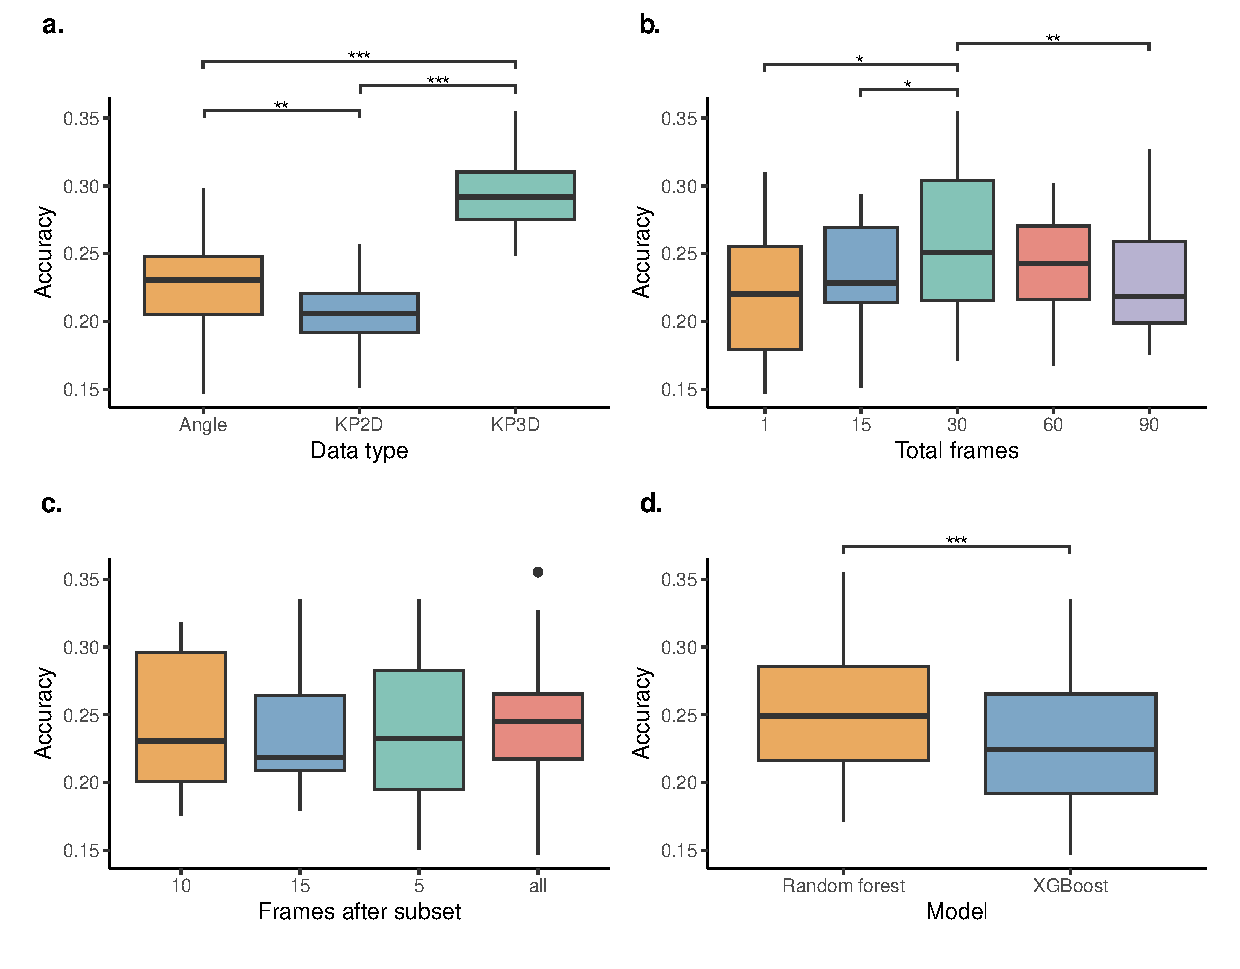
\includegraphics[width=1\linewidth]{results_boxplot_final.pdf}
    \caption{Results of Tukey HSD test pairwise comparisons, depicting the within group differences for different \textbf{a.} data types, \textbf{b.} total frame lengths, \textbf{c.} frame lengths after subsetting, and \textbf{d.} models. Asterisks represent significant differences between groups that were detected for the Tukey HSD test (*: p $<$ 0.05, **: p $<$ 0.01, ***: p $<$ 0.001.)}
    \label{fig:results_boxplot}
\end{figure}


    \noindent The data from 37 trials were used for analysis, of which 22 contained 2 pigeons, 10 contained 5 pigeons, and 5 contained 10 pigeons, corresponding to 1,208,728 total frames of data.
    %
    Sample size was limited by the number of consecutive frames of grooming, the behaviour with the fewest samples found. For 90 continuous frames of grooming, a maximum of 210 and 35 samples were found for the training and testing sets respectively. All other behaviours at all other frame lengths were therefore also sampled according to this sample size, balancing the different behavioural classes. \\
    
    % -------------------------------------------------------------------- %
    
    \noindent The best performing model and data combination was found to be the random forest model trained on 30 frames of 3D keypoint data that was not further subsetted (Table \ref{results_table}). This reached an accuracy score of 0.355, equivalent to predicting 35.5\% of all test samples correctly. A confusion matrix was constructed to depict the prediction the model made for each behaviour (Figure \ref{fig:confusion_matrix}). The hyperparameters used in the grid search for model optimisation included the maximum depth of the trees (max\_depth), the minimum number of samples required to split an internal node (min\_samples\_split), the maximum number of terminal nodes on a tree (max\_leaf\_nodes), and the minimum number of samples each terminal node contains (min\_samples\_leaf). The grid search optimised model however achieved an accuracy score of 0.347 on the testing set, lower than the initial model, on the hyperparameters ``max\_depth = 10", ``max\_leaf\_nodes = 120", ``min\_samples\_leaf = 4" and ``min\_samples\_split = 2". The same model however achieved an accuracy score of 0.869 on the training set, indicating overfitting of the model to the training set. 5-fold cross validation returned a mean standard deviation of 0.021. \\
    
    \noindent The mean accuracy score differed significantly between all data types. The accuracy of models trained on 3D keypoint data was significantly higher than both angle data (difference: 0.068, CI: ±0.015, p $<$ 0.001) and 2D keypoint data (difference: 0.089, CI: ±0.015, p $<$ 0.001). The accuracy of models trained on angle data was significantly higher than 2D keypoint data (difference: 0.021, CI: ±0.015, p $<$ 0.01).
    %
    A frame size of 30 yielded the highest average accuracy score, which was significantly higher than the scores for 1 frame (difference: 0.038, CI: ±0.016, p $<$ 0.05), 15 frames (difference: 0.029, CI: ±0.014, p $<$ 0.05), and 90 frames (difference: 0.028, CI: ±0.020, p $<$ 0.01). However, the accuracy score for 30 frames was not significantly different from that for 60 frames. Overall, average accuracy scores tended to decrease as the frame size moved away from 30, either increasing or decreasing.
    %
    There was no significant difference between the different frame sizes after subsetting, and all yielded comparable accuracy scores.
    %
    The random forest models were found to yield significantly higher accuracy scores than the XGBoost models (difference: 0.020, CI: ±0.010, p $<$ 0.001) (figure \ref{fig:results_boxplot}).\\

    
%                  diff          lwr          upr     p adj
%30-1   0.038095238  0.006216336  0.069974140 0.0110421 *
%30-15  0.028571429  0.003878137  0.053264720 0.0150935 *
%90-30 -0.027551020 -0.047713008 -0.007389032 0.0024348 **

%                  diff         lwr          upr     p adj
%KP2D-Angle -0.02122449 -0.03665407 -0.005794914 0.0042867 **
%KP3D-Angle  0.06802721  0.05259764  0.083456786 0.0000000 ***
%KP3D-KP2D   0.08925170  0.07382213  0.104681276 0.0000000 ***

%              diff         lwr          upr     p adj
% xg-rf -0.01995465 -0.03045255 -0.009456744 0.0002994 ***


    % ---------------------------------------------------------------------%
    \noindent A maximum of 1200 samples could be found for each behaviour when sampled using a frame size of 30. The prediction accuracies for the random forest and XGBoost models started at a baseline of 0.155 and 0.143 respectively with a sample size of 1, comparable to the probability of randomly predicting 1/7 behaviours. The prediction accuracy for both models increase as the sample size increases from 1, and plateaus at 0.353 and 0.337 respectively. The random forest model reaches this plateau point quicker than the XGBoost model (figure \ref{fig:model_performance}).
    
    \begin{figure}[htbp]
        \centering
        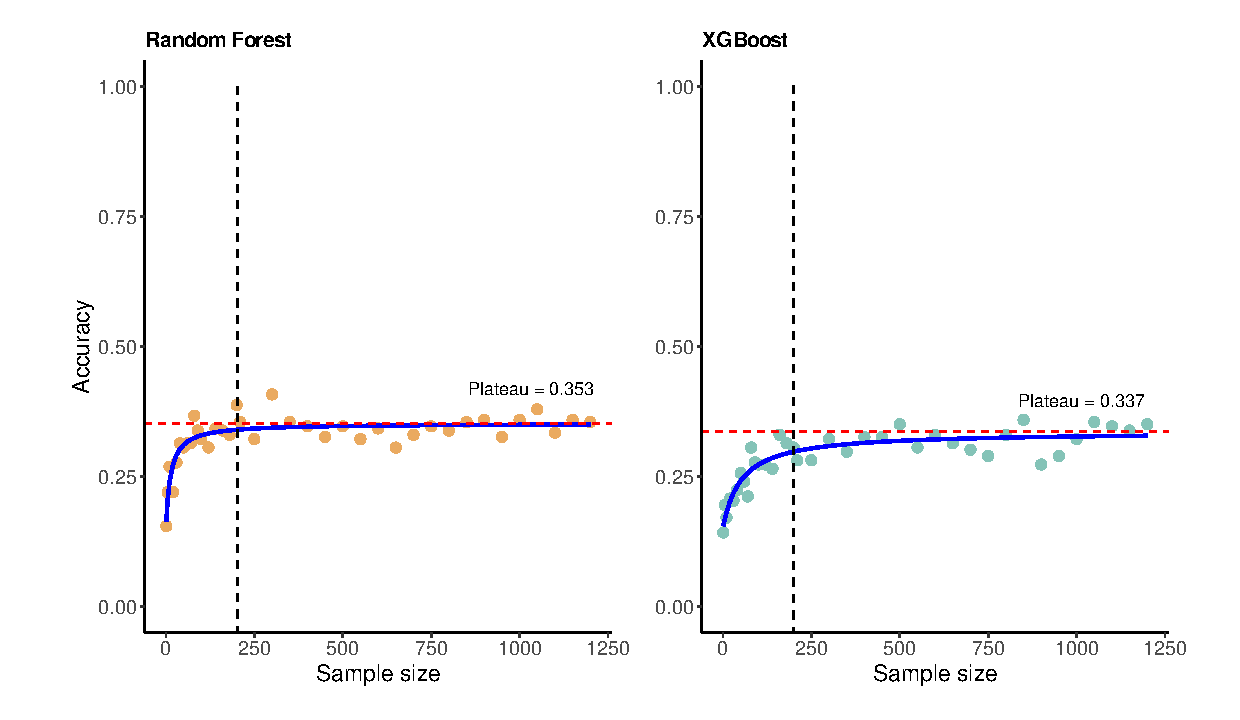
\includegraphics[width=1\linewidth]{model_performance_plot.pdf}
        \caption{Model performance of the random forest and XGBoost models trained on 30 frames of non-subsetted 3D keypoint data, when trained with different sample sizes. The blue curve is the asymptotic regression curve, and the red dotted line is the plateau value, the maximum predicted accuracy for the model. The black vertical dotted line represents a sample size of 210, which is the training dataset size of this study.}
        \label{fig:model_performance}
    \end{figure}

    
    \begin{figure}[htbp]
        \centering
        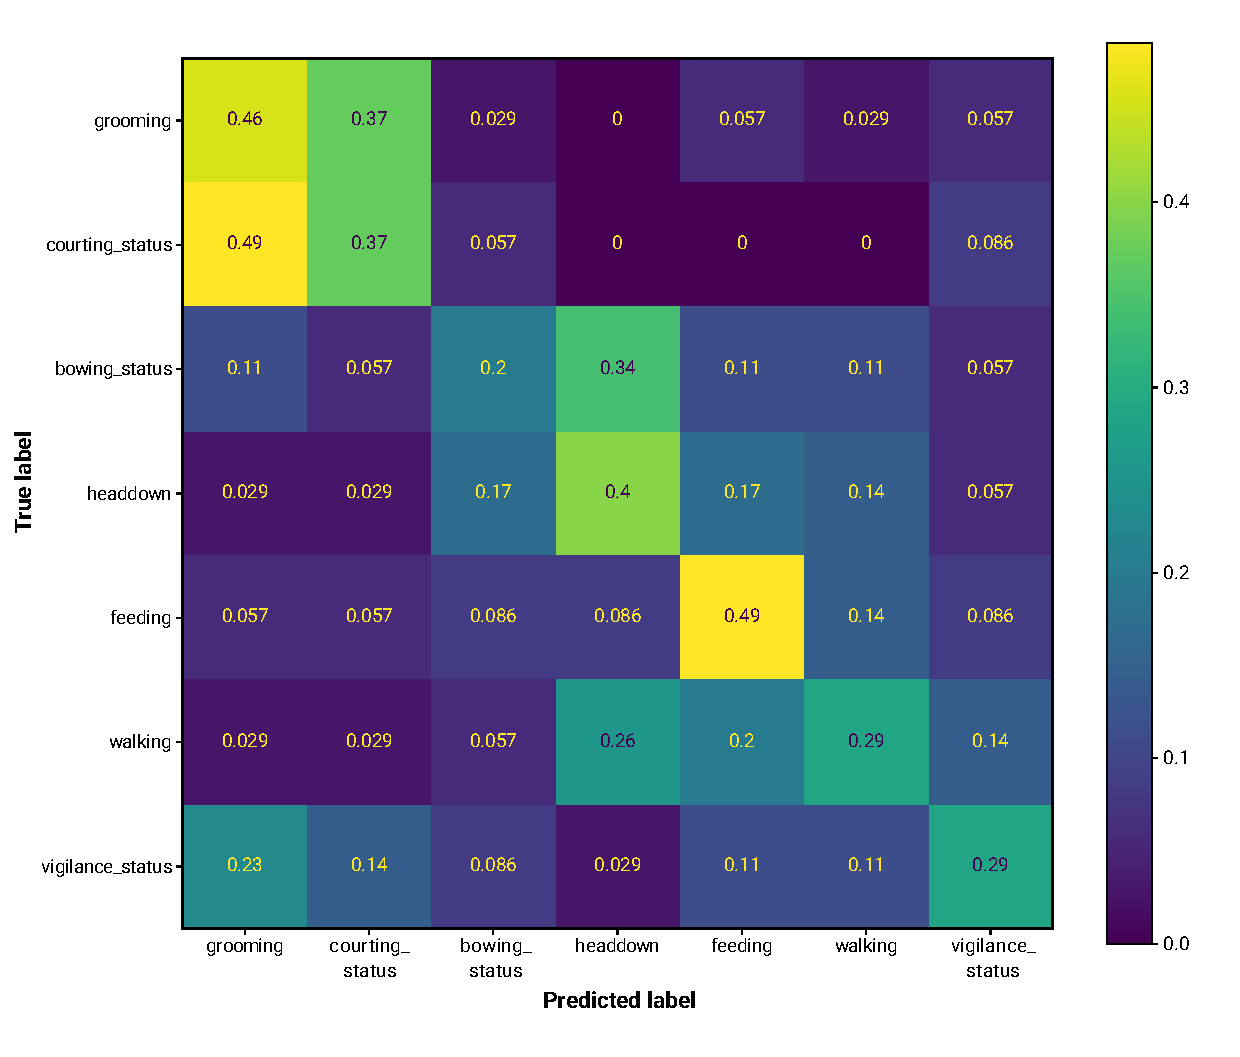
\includegraphics[width=1\linewidth]{CF_rf3030.pdf}
        \caption{Confusion matrix for the random forest model trained on 30 frames of non-subsetted 3D keypoint data. Numbers represent percentage chance that a true label is given a predicted label.}
        \label{fig:confusion_matrix}
    \end{figure}






% ---------------------------------------------------------------- %
%%%%%%%%%%%%%%%%% DISCUSSION %%%%%%%%%%%%%%%%%%%%%%%%%%%%%%%%%%%%%%%%%
% ---------------------------------------------------------------- %
\newpage
\section{Discussion}

In this study, I compared posture data of different data types, frame lengths and subsetted frame lengths, for use in the classification of pigeon behaviours using two machine learning algorithms. 
%
My findings highlight the advantages of using both 3D keypoint and time frame data over 1-2 seconds for pigeon behaviour classification, indicating the potential of using such data in future studies in the field of animal behaviour classification, despite the increased challenges in obtaining data in these formats.
%
However, these results are complicated by low prediction accuracy which was found for all models. The low accuracy suggests that the data I used could be unsuitable for behaviour prediction, due to the high dimensionality and low explanatory power of input data. Low accuracy could also point to shortcomings in the machine learning models, which means the data cannot be analysed effectively. Limitations could include the models being unsuited for processing time series data, and overfitting to the training set. Due to this low overall accuracy, my results should be interpreted with caution. \\



\subsection{Differences between posture estimation data types}
\noindent The largest difference in accuracy score was found between the different types of data, where 3D keypoints were found to have a significantly higher accuracy score compared to both 2D keypoints and angles. This suggests that despite the higher requirements of obtaining 3D keypoints, doing so could lead to better predictions overall. One reason for the better performance of 3D keypoints here could be that they are consistent in information captured regardless of the posture or direction a pigeon is facing, whereas 2D keypoints would capture different information from the same scene, depending on the angle and perspective the camera is viewing from, and the orientation of the pigeon. Another reason could be the reduction of occlusions for 3D data compared to 2D, especially for complex scenes involving multiple animals or obstructions. 3D data also captures a greater range of motion and dynamic poses in animals compared to 2D data, and is more suitable in characterising keypoints on limbs \citep{datta_computational_2019}. Although not applicable to 3D-POP, this could be important for datasets where limbs are involved, or the tracked animal exhibits more dynamic motions. 
%
The reason for 3D keypoint data outperforming angle data could be due to the angle data being simplified too much, and therefore representing a smaller amount of information compared to the original 3D keypoints. In my study, angles only described the relative position of the head and body of the pigeon, whereas the physical distance between the two, the length of the neck, is lost. The neck of birds is highly flexible and maneuverable, and can act as an appendage to enable many behaviours \citep{neck_2023} including bowing, grooming and pecking, all of which assume different neck postures. \citet{human_angles_2020} used the angles as well as the vector distances between joints to approximate human postures during exercise, potentially indicating the need to calculate distances between joint angles. Future study could investigate if including the distance between angles can improve prediction accuracy. \\

\noindent Although 3D keypoints hold great potential, the greatest difficulty is still the lack of sufficient annotated 3D data for any given animal species. With marker-based motion capture set-ups such as for 3D-POP \citep{naik_3d-pop_2023}, although pigeons were able to behave normally with attachments on the body, attachments may not be suitable for animals such as macaques (\textit{Macaca mulatta}), which are agile enough to remove markers, and show discomfort with them on \citep{3D_macaque_2020}. Furthermore, a motion capture system requires extensive specialist hardware and software to function, limiting its use anywhere outside of a specialised lab. The challenges of using marker-based motion capture means high quality 3D keypoint datasets are difficult to obtain. 
% Many large human 3D keypoint datasets exist, and were also generated using motion capture systems \citep{2D3Dkp_review_2021}. 
%
This difficulty could be resolved by deep learning techniques, which have allowed for the rise of markerless keypoint detection methods \citep{deep_mocap_2020, mathis_deeplearning_2020}. Methods such as DeepLabCut \citep{mathis_deeplabcut_2018} can use two camera views to triangulate the position of 3D keypoints from their 2D counterparts, which can be automatically predicted using small manually labelled datasets \citep{deeplabcut_3D_2019}. Advancements in deep learning have also meant that only a single camera view can generate 3D keypoints in some cases, using either 2D keypoints or a heatmap as an intermediate step \citep{liftpose3d_2021, monocular_2022}. These methods do not need specialised motion capture setups or attachments on an animal's body, and can be used in diverse settings including in the field, with a variety of animal species \citep{3D_macaque_2020, joska_acinoset_2021, 3D_monkey_2023}. For example, \citet{joska_acinoset_2021} was able to generate a large dataset of 3D keypoints for cheetahs (\textit{Acinonyx jubatus}) running in the field by capturing 2D keypoints at multiple angles to generate 3D keypoints, demonstrating the potential of using 3D keypoint annotation beyond specialised lab settings, and applicability to more animal species.
%
However, although these methods do not require extensive human-labelled data for prediction, human-labelled data is still required to evaluate the accuracy of the automatic keypoint predictions \citep{waldmann_3d-muppet_2023}. Additionally, as they derive 3D keypoints from corresponding 2D keypoints, these methods are still vulnerable to occlusions, or other problems encountered when sourcing the 2D points \citep{deeplabcut_3D_2019,monocular_2022}.

    % ---------------------------------------------------------------------%

\subsection{Differences between total time frame sizes}
Models trained on 30 total frames outperformed models trained on 1, 15 and 90 total frames, whilst being equivalent to 60 frames. This suggests that 30-60 frames of data, equivalent to 1-2 seconds of footage, was best suited to capture pigeon behaviours in the 3D-POP dataset, and could be the time scale at which the behaviours of pigeons are best predicted. Time scales greater than 1-2 seconds could represent too much information, whereas time scales smaller than this could mean the behaviour sequences are not fully captured, or not captured at all for single stationary frames.
%
Several previous animal studies have made use of time series data to predict animal behaviour, and have found a similar trend of an optimal time frame, with poorer performance as the time frame becomes longer or shorter \citep{sheep_timeseries_2018, RNN_window_2019}.
%
Human behaviour recognition has also produced similar findings. A broad range of time frames from 0.1 second to more than 10 seconds have been tested in numerous studies, but time frames of 2 seconds or less were found to yield most accurate predictions overall, suggesting that short sequences contain sufficient information to predict behaviours, whilst longer sequences could contain too much information and noise for accurate predictions \citep{banos_window_2014}. \\

\noindent Repetitive motions of pigeons such as head bobbing, pecking and bowing, characteristic of behaviours such as walking, feeding and courting, could potentially occur within a time scale of 1-2 seconds, and be detected by the machine learning algorithms \citep{head-bobbing_1988, shimizu_conspecific_1998, ware_social_2017}. Alternatively, the algorithms could detect more fine scale movements that are not as easy to identify by eye, but forms part of a behaviour. Several recent techniques have utilised unsupervised methods to identifying these discrete motifs (also called modules or syllables) of behaviour, instead of the full 'behaviours' as defined by humans \citep{hsu_b-soid_2021, keypoint-moseq_2024}. These motifs of behaviour found by unsupervised methods often represent short motions or repetitive movements, and are typically much shorter in duration compared to what humans would consider a behaviour in manual definition, lasting between 0.033 - 0.4 seconds depending on the technique and resolution of data \citep{keypoint-moseq_2024}. Depending on the time scale in use, different motifs can be identified \citep{fly_timeseries_2019}. 
%
This presents an opportunity to investigate if these unsupervised methods and time frames for motifs can be generalised to birds, given that these methods are usually tested on invertebrates and rodents. Breaking down of behaviours into finer motifs could prove advantageous to behavioural prediction of pigeons and other species, where algorithms could be fine tuned to detect combinations of motifs, potentially increasing prediction accuracy \citep{luxem_identifying_2022, fazzari_animal_2024}. 


    % ---------------------------------------------------------------------%

\subsection{Effect of dimensionality reduction}
There was no significant difference between the prediction accuracy of different time frame subsets, suggesting that both the full and reduced samples performed similarly, and that consecutive frames do not provide additional information to the model overall. This finding highlights issues with high dimensionality, namely that full samples might contain redundant features that contribute little to the overall model performance, and make it difficult for the model to identify important features within a vast feature set \citep{curse_2005}. Indeed, each 3D keypoint corresponds to its x, y and z coordinate values, meaning a set of 9 keypoints corresponds to 27 input features. For 90 frames of 3D keypoints, this would result in a very high 2430 input features for the model.
%
However, the fact that subsetted models did not perform better than the full models suggests that the remaining features were not more informative than the original set, implying that the dimensionality of the remaining features may still be too high, or that collinear features were not eliminated. The low accuracy scores observed across all models further support this concern.
%
High dimensionality could also explain the severe overfitting that was found in all models I fit, where prediction accuracy on the training set was extremely high, whereas the test set accuracy was low, suggesting that models are unable to generalise to data beyond the training dataset. Increasing number of features increases the flexibility of the models when fitting the data, which may lead to overfitting as the models not only fit to identified patterns, but also random noise in the training sample \citep{curses_2018}. 
%
Classic dimensionality reduction methods such as principal component analysis (PCA) could be used to reduce the number of features (dimensions) used for prediction, whilst summarising them into fewer features that contain more explanatory power each. This offers a way for datasets with large numbers of features to be used without issues such as overfitting arising.



    % ---------------------------------------------------------------------%

\subsection{Differences between models}
Random forest models achieved significantly higher predictive accuracy scores compared to XGBoost, but the difference between them was small. Indeed, accuracy scores for random forest and XGBoost are usually similar for behaviour classification tasks, with \citet{bergen_review_2023} finding XGBoost to be slightly better at eagle behaviour classification after 2 rounds of hyperparameter tuning, but \citet{yu_evaluation_2021} finding performance of both models to be indiscernible across the behaviour classification of multiple species. Random forest could have outperformed XGBoost in my study because it is more robust to overfitting compared to XGBoost. This robustness comes from random forest being an ensemble method, whereas XGBoost performs gradient boosting on top of being an ensemble method. Ensemble methods create many uncorrelated decision trees using random subsets of the training data, where this introduced randomness and use of only part of the total data minimising overfitting \citep{ML_for_behaviour_2017, bentejac_comparative_2021, bergen_review_2023}. Gradient boosting methods however build sequential trees which correct upon the errors of the previous tree \citep{bentejac_comparative_2021,bergen_review_2023}, and can be prone to overfitting especially when data is complex and noisy, requiring greater fine tuning of hyperparameters to mitigate such problems. Indeed, the un-optimised XGBoost model has been found to under-perform compared to other models, suggesting that future studies with optimised models could see better prediction results \citep{bentejac_comparative_2021}.\\

\noindent Unlike the findings of \citet{bergen_review_2023} and \citet{yu_evaluation_2021} however, the predictive accuracy was low across all models in my study. One reason for this could be that both the random forest and XGBoost models struggled to effectively process the time series data, leading to a loss of the temporal component within the samples. This is apparent in the variation of frame lengths: although different frame lengths represented different durations of time, and significant differences were found between some of them, these differences remained small. This could suggest that despite inputting a time series of frames, the models treated the contents of each frame independently, rather than recognizing their sequential relationships as part of a time series. As a result, the analysis may have overlooked posture changes and movement from one frame to the next. This inherent limitation could also explain why increasing sample size only increased model performance up to a point, after which performance no longer increased with more samples (figure \ref{fig:model_performance}). To allow better analysis of time series data, alternative models such as recurrent neural networks (RNN) could be used, which is a deep learning model that natively supports the prediction of sequential data such as time series, and can use their neural network properties to deduce complex patterns in data \citep{timeseries_book}. Long Short-Term Memory (LSTM) models are a powerful type of RNN that builds on to the classic RNN's capabilities by allowing memorisation of data in long sequences \citep{timeseries_book}, making it highly suitable for analysis of data such as multiple consecutive frames of pigeon movement keypoints. However, large samples sizes are required for the training of RNN models, and future studies will have to employ alternative methodologies to obtain larger numbers of data samples from the 3D-POP dataset or elsewhere, or to pre-train the model on alternative larger datasets using techniques such as transfer learning \citep{mathis_deeplearning_2020, sagheer_deep_2021}.






% ---------------------------------------------------------------- %
%%%%%%%%%%%%%%%%% CONCLUSION %%%%%%%%%%%%%%%%%%%%%%%%%%%%%%%%%%%%%%%%%
% ---------------------------------------------------------------- %

\section{Conclusion}

\noindent This study finds that estimating posture of pigeons using 3D keypoints results in better machine learning accuracy compared to using 2D keypoints or angles, providing evidence to support the use of 3D posture estimation in animal behaviour studies - a field that is currently lacking in both large 3D keypoint datasets and frameworks to generate them, but can benefit greatly from the increased  This study also finds that 1-2 seconds of data results in better prediction accuracy compared to longer or shorter time frames, providing support for the use of short time frames for behaviour detection, and evidence for the time scale that defines repeating behaviours in pigeons. Despite these findings, overall prediction accuracy was low across all models, indicating potential limitations of the models used, the input data, or both. The input data was of very high dimensionality for all models, suggesting that dimensionality reduction methods may be required to improve model accuracy. The random forest model outperformed XGBoost, but both models had poor prediction accuracy, suggesting that alternative models such as recurrent neural networks could be used instead to better analyse time series data. Findings of this study should be taken with this low accuracy in mind.



% ---------------------------------------------------------------- %
%%%%%%%%%%%%%%%%% ACKNOWLEDGEMENTS %%%%%%%%%%%%%%%%%%%%%%%%%%%%%%%%%
% ---------------------------------------------------------------- %
\newpage
\section*{Acknowledgements}
I would like to thank my supervisor Alex Chan for helping me develop my project, providing excellent resources for reading, giving patient explanations for when I had questions, and providing me with hospitality during my stay at the University of Konstanz. I would like to thank the lab group of Dr. Fumihiro Kano at the University of Konstanz for their valuable suggestions reagarding my project. I would like to thank my supervisor Dr. Julia Schroeder for her extensive and valuable feedback given during mock presentations, and the weekly lab meetings with her group. I would like to thank the members of Julia's lab group for their feedback and suggestions for my project. I would like to thank Jianing Ge and Haoyue Zhang for reading and discussion my project with me on many occasions. 

\section*{Code and Data Availability}
All code and data used in this project can be found in the following Github repository: \\ https://github.com/TianlePotato/CMEE\_project


% ---------------------------------------------------------------- %
%%%%%%%%%%%%%%%%% REFERENCES %%%%%%%%%%%%%%%%%%%%%%%%%%%%%%%%%%%%%%%
% ---------------------------------------------------------------- %
\newpage
\section*{References}

    \nocite{brown_accelerometer_finescale_2013}
    \nocite{c_elegans_2013}

\begingroup
\renewcommand{\section}[2]{}%
\bibliography{references}
\endgroup


\end{document}
